\section{Applying the default group sequential design\label{sec:default}}
\subsection{Default parameters}
We are now prepared to demonstrate derivation of group sequential designs using default parameters with the \code{gsDesign()} function.
Along with this, we discuss the \texttt{gsDesign} class returned by \texttt{gsDesign()} and its associated standard print and plot functions. 
We then apply this default group sequential design to each of our motivational examples. 
The main parameters in \code{gsDesign()} will be explained in more detail in sections \ref{sec:gsDesign} through \ref{sec:spendfn}.

The main parameter defaults that you need to know about are as follows:

\begin{enumerate}
\item Overall Type I error $\alpha = 0.025$ (one-sided)

\item Overall Type II error $\beta = 0.1$ (Power = $90\%$)

\item Two interim analyses equally spaced at 1/3 and 2/3 of the way through the trial plus the final analysis (\texttt{k=3})

\item Asymmetric boundaries, which means we may stop the trial for futility or
superiority at an interim analysis.

\item $\beta$-spending is used to set the lower stopping
boundary. This means that the spending function controls the incremental
amount of Type II error at each analysis, $\beta_i(\delta)$, $i=1,2,\ldots,K$.

\item Non-binding lower bound. Lower bounds are sometimes considered as
guidelines, which may be ignored during the course of the trial. 
Since Type I error is inflated if this is the case, regulators often demand that the lower bounds be ignored when computing Type I error.
That is, Type I error is computed using $\alpha^+(\theta)$ from (\ref{alphai+(theta)}) and (\ref{alpha+(theta)}) rather than $\alpha(\theta)$ from (\ref{alphai(theta)}) and (\ref{alpha(theta)}). 

\item A Hwang-Shih-DeCani spending functions with $\gamma = -4$ for the upper
bound and $\gamma = -2$ for the lower bound. This provides a conservative,
O'Brien-Fleming-like superiority bound and a less conservative lower bound.
Spending functions will be discussed in detail in \ref{sec:spendfn}.
\end{enumerate}

\subsection{Sample size ratio for a group sequential design compared to a fixed
design.\label{sec:ssratio}}

In section \ref{sec:testing} and its subsections we gave distributional assumptions, defined testing procedures and denoted probabilities for boundary crossing.
Consider a trial with a fixed design (no interim analyses) with power 100(1--$\beta$) and level $\alpha$ (1-sided). Denote the sample size as $N_{fix}$ and statistical information for this design as $I_{fix}$. 
For a group sequential design as noted above, we denote the information ratio (inflation factor) comparing the information planned for the final analysis of a group sequential design compared to a fixed design as
\begin{equation}
r=I_{k}/I_{fix}=n_{k}/N_{fix}.\label{ssratio}%
\end{equation}
This ratio is independent of the $\theta$-value $\delta$ for which the trial
is powered as long as the information (sample size) available at each analysis
increases proportionately with $I_{fix}$ and the boundaries for the group
sequential design remain unchanged; see, for example, Jennison and Turnbull \cite{JTBook}. 
Because of this, the default for \texttt{gsDesign()} is to print the sample size ratios $r_i=I_i/I_k$, $i=1,2,\ldots,k$ rather than an actual sample size at each interim analysis. 
This is implemented through by the default value of 1 for the input parameter \texttt{n.fix}. 
We demonstrate in the following subsections how to set \texttt{n.fix} to apply to our motivating examples.

\subsection{The default call to \texttt{gsDesign()}}
We begin with the call 
\verb!x <- gsDesign()!
to generate a design using all default arguments. The next line
prints a summary of \texttt{x}; this produces the same effect as
\texttt{print(x)} or \texttt{print.gsDesign(x)}. Note that while the total
Type I error is $0.025$, this assumes the lower bound is ignored if it is
crossed; looking lower in the output we see the total probability of crossing
the upper boundary at any analysis when the lower bound stops the trial is
$0.0233$. Had the option 
\verb!x <- gsDesign(test.type=3)!
been run, both of these numbers would assume the trial
stops if the lower bound stopped and thus would both be $0.025$. 

\bigskip

\begin{verbatim}
> x <- gsDesign()
> x
Asymmetric two-sided group sequential design with 90 % power and 2.5
Type I Error.
Upper bound spending computations assume trial continues if lower bound is
crossed.

           Sample
            Size    ----Lower bounds----  ----Upper bounds-----
  Analysis Ratio*   Z   Nominal p Spend+  Z   Nominal p Spend++
         1  0.357 -0.24    0.4057 0.0148 3.01    0.0013  0.0013
         2  0.713  0.94    0.8267 0.0289 2.55    0.0054  0.0049
         3  1.070  2.00    0.9772 0.0563 2.00    0.0228  0.0188
     Total                        0.1000                 0.0250 
+ lower bound beta spending (under H1): Hwang-Shih-DeCani spending function 
  with gamma = -2
++ alpha spending: Hwang-Shih-DeCani spending function with gamma = -4
* Sample size ratio compared to fixed non-group sequential design

Boundary crossing probabilities and expected sample size assuming any cross
stops the trial

Upper boundary (power or Type I Error)
          Analysis
   Theta      1      2      3  Total   E{N}
  0.0000 0.0013 0.0049 0.0171 0.0233 0.6249
  3.2415 0.1412 0.4403 0.3185 0.9000 0.7913

Lower boundary (futility or Type II Error)
          Analysis
   Theta      1      2      3  Total
  0.0000 0.4057 0.4290 0.1420 0.9767
  3.2415 0.0148 0.0289 0.0563 0.1000

> plot(x)
\end{verbatim}
\begin{figure}
\begin{center}
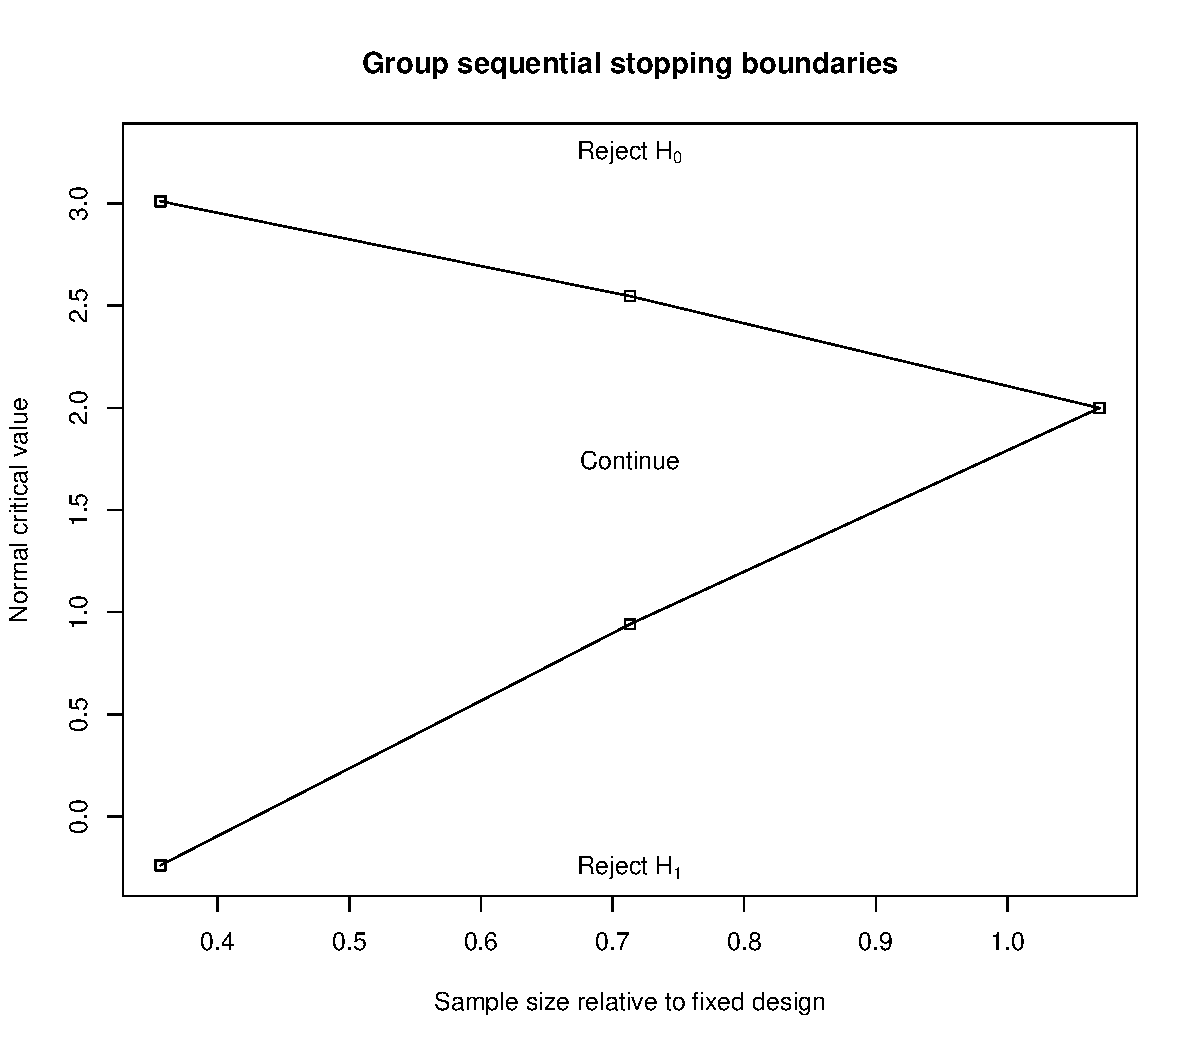
\includegraphics[width=.6\textwidth]{figs/boundplot.pdf}
\end{center}
\caption{Default plot for gsDesign object}
\end{figure}%

\bigskip

Above we have seen standard output for \texttt{gsDesign()}. 
To access individual items of information about what is returned from the above, use \texttt{summary(x)} to list the elements of \texttt{x}.
Type \texttt{help(gsDesign)} to get full documentation of the class \texttt{gsDesign} returned by the \texttt{gsDesign()} function. 
To view an individual element of \texttt{x} type, for example, \texttt{x\$delta}. 
Other elements of \texttt{x} can be accessed in the same way, and we will use these to display aspects of designs in further examples. 
Of particular interest are the elements \texttt{upper} and \texttt{lower}. 
These are both objects containing multiple variables concerning the upper and lower boundaries and boundary crossing probabilities.
Type \texttt{summary(x\$upper)} to show what these variables are. 
The upper boundary can be shown with the command \texttt{x\$upper\$bound}.
For additional plots, enter \texttt{plot(x, plottype=2))} for a power plot.
The argument \texttt{plottype} can run from 1 (the default) to 7.
The options not already noted plot effect sizes at boundaries (\texttt{plottype=3}), conditional power at boundaries (\texttt{plottype=4})), 
$\alpha$- and $\beta$-spending functions (\texttt{plottype=5})), expected sample size by underlying treatment difference (\texttt{plottype=6}), and B-values at boundaries (\texttt{plottype=7}).

\subsection{Applying the default design to the CAPTURE example}
The sample size ratios from (\ref{ssratio}) can be obtained as follows:
\begin{verbatim}
> x <- gsDesign()
> x$n.I
[1] 0.3566277 0.7132554 1.0698832
\end{verbatim}
These will be applied to each of our examples.
Recall from the CAPTURE trial that we had a binomial outcome and wished to detect a reduction in the primary endpoint from a 15\% event rate in the control group to a 10\% rate in the experimental group.
While we consider 80\% power elsewhere, we stick with the default of 90\% here.
A group sequential design with 90\% power and 2.5\% Type I error has the same bounds as shown previously. The sample size at each analysis is obtained as follows (continuing the code just above):
\begin{verbatim}
> n.I <- nBinomial(p1 = .15, p2 = .1)
> n.I
1834.641
> n.I * x$n.I
[1]  654.2839 1308.5679 1962.8518
\end{verbatim}
Rounding up to an even number in each case, we see from the above that a while a fixed design requires 1836 patients, employing the default group sequential design inflates the sample size requirement to 1964. 
Interim analyses would be peformed after approximately 654 and 1308 patients.

The group sequential design can be derived directly by replacing the input parameter \texttt{n.fix} with the sample size from a fixed design trial as follows:

\begin{verbatim}
> n.I <- nBinomial(p1 = .15, p2 = .1)
> x <- gsDesign(n.fix = n.I)
> x$n.I
[1]  654.2839 1308.5678 1962.8518
\end{verbatim}

Printing this design now replaces the sample size ratio with the actual sample sizes at each analysis. The only other difference from the design above in Section \ref{sec:default} is the second value of \texttt{theta} below.

\begin{verbatim}
> x
Asymmetric two-sided group sequential design with 90 % power and 
2.5 % Type I Error.
Upper bound spending computations assume trial continues if lower 
bound is crossed.

                  ----Lower bounds----  ----Upper bounds-----
  Analysis   N    Z   Nominal p Spend+  Z   Nominal p Spend++
         1  655 -0.24    0.4057 0.0148 3.01    0.0013  0.0013
         2 1309  0.94    0.8267 0.0289 2.55    0.0054  0.0049
         3 1963  2.00    0.9772 0.0563 2.00    0.0228  0.0188
     Total                      0.1000                 0.0250 
+ lower bound beta spending (under H1): Hwang-Shih-DeCani spending 
function with gamma = -2
++ alpha spending: Hwang-Shih-DeCani spending function with gamma = -4

Boundary crossing probabilities and expected sample size assuming 
any cross stops the trial

Upper boundary (power or Type I Error)
          Analysis
   Theta      1      2      3  Total   E{N}
  0.0000 0.0013 0.0049 0.0171 0.0233 1146.4
  0.0757 0.1412 0.4403 0.3185 0.9000 1451.7

Lower boundary (futility or Type II Error)
          Analysis
   Theta      1      2      3  Total
  0.0000 0.4057 0.4290 0.1420 0.9767
  0.0757 0.0148 0.0289 0.0563 0.1000
\end{verbatim}

\bigskip

\subsection{Applying the default design to the noninferiority example}
The fixed noninferiority design for a binomial comparison is the same as above, only changing the \texttt{nBinomial()} call to 
\bigskip
\begin{verbatim}
> n.fix <- nBinomial(p1=.677, p2=.677, delta0=.07)
> ceiling(gsDesign(n.fix = n.fix)$n.I)
[1]  668 1336 2004
>\end{verbatim}
\bigskip
Testing at each analysis can be peformed using the Miettinen and Nurminen \cite{MandN} method.
Simulation to verify the normal approximation is adequate for comparing binomial event rates can be performed using the functions \code{simBinomial} and \code{testBinomial}.

\subsection{Applying the default design to the cancer trial example}
For trials with time-to-event outcomes, the variable \texttt{n.fix} in \texttt{gsDesign()} needed is the number of events from a fixed design trial. 
The reader may wish to refer to Jennison and Turnbull \cite{JTBook} for further background; we also discuss distributional assumptions further in Section \ref{sec:TTE}.
We begin with the code from the fixed design trial for the cancer trial example from \ref{sec:CAex}.
Next, we call to \code{gsDesign()} with \texttt{n.fix} equal to the number of events for a fixed trial design. 
The value \code{ssratio}, the sample size ratio at each analysis compared to the fixed design sample size is then shown. Note that the values are the same as shown in the first output of this example above.
The inflation in the total sample size is the same as for the number of events required; that is, the sample size required for a group sequential design with the default interim analysis plan is inflated to 595 (or 596 for an even number) from 557 (or 558) from that of a fixed design by multiplying by 1.07. 

\begin{verbatim}
> x <- nSurvival(lambda.0=log(2)/6,lambda.1=log(2)/6*.7,eta=-log(.95),
+         Tr=30,Ts=36,type="rr",entry="unif")
> ceiling(x$Sample.size)
[1] 557
> ceiling(x$Num.events)
[1] 330
> y <- gsDesign(n.fix=x$Num.events)
> ceiling(y$n.I)
[1] 118 236 353
> ssratio <- (y$n.I / x$Num.events)
> ssratio
[1] 0.3566277 0.7132554 1.0698831
> ceiling(ssratio[3] * x$Sample.size)
[1] 595
\end{verbatim}

\subsection{Using \texttt{gsProbability()} following \texttt{gsDesign()}}

We reconsider the default design and obtain the properties for a larger
set of $\theta$ values than in the standard printout for \texttt{gsDesign()} shown previously.
The first two lines of code below demonstrates a group sequential design generated by \texttt{gsDesign()} can be input to \texttt{gsProbability()} to obtain boundary crossing probabilities for an extended set of parameter values.
The \texttt{theta} values in the output make more sense in this case when they are computed relative to the effect size \texttt{x\$delta} for which the trial is powered; this is more easily seen in the plot of expected sample size shown here since the $x$-axis uses this scale. 
Note that the $y$-axis shows the expected sample size relative to a fixed design trial when the sample size ratio is computed; if we had input a fixed design sample size, the $y$-axis would show the actual expected sample size.
Note further that the \texttt{plot()} function for the \texttt{gsDesign} class (used here) is an extension of the standard \texttt{plot()} function, and thus allows use of many of its parameters, such as line width (\texttt{lwd}), line type (\texttt{lty}), plot titles and axis labels.
This plot demonstrates the ability of a group sequential design to appropriate adapt sample size to come to an appropriate conclusion depending on the true treatment effect. If the effect size is twice that for which the trial is powered, the expected sample size is about 40\% of that for a fixed design, compared to over 80\% in some cases when the true treatment effect is between the hypothesized values for the efficacy parameter $\theta$. 

\bigskip

\begin{verbatim}
> x <- gsDesign()
> y <- gsProbability(theta=x$delta*seq(0, 2, .25), d=x)
> y 
Asymmetric two-sided group sequential design with 90 % power and 
2.5\% Type I Error.
Upper bound spending computations assume trial continues if lower bound is 
crossed.

           Sample
            Size    ----Lower bounds----  ----Upper bounds-----
  Analysis Ratio*   Z   Nominal p Spend+  Z   Nominal p Spend++
         1  0.357 -0.24    0.4057 0.0148 3.01    0.0013  0.0013
         2  0.713  0.94    0.8267 0.0289 2.55    0.0054  0.0049
         3  1.070  2.00    0.9772 0.0563 2.00    0.0228  0.0188
     Total                        0.1000                 0.0250 
+ lower bound beta spending (under H1): Hwang-Shih-DeCani spending function
with gamma = -2
++ alpha spending: Hwang-Shih-DeCani spending function with gamma = -4
* Sample size ratio compared to fixed non-group sequential design

Boundary crossing probabilities and expected sample size assuming any cross 
stops the trial

Upper boundary (power or Type I Error)
          Analysis
   Theta      1      2      3  Total   E{N}
  0.0000 0.0013 0.0049 0.0171 0.0233 0.6249
  0.8104 0.0058 0.0279 0.0872 0.1209 0.7523
  1.6208 0.0205 0.1038 0.2393 0.3636 0.8520
  2.4311 0.0595 0.2579 0.3636 0.6810 0.8668
  3.2415 0.1412 0.4403 0.3185 0.9000 0.7913
  4.0519 0.2773 0.5353 0.1684 0.9810 0.6765
  4.8623 0.4574 0.4844 0.0559 0.9976 0.5701
  5.6727 0.6469 0.3410 0.0119 0.9998 0.4868
  6.4830 0.8053 0.1930 0.0016 1.0000 0.4266

Lower boundary (futility or Type II Error)
          Analysis
   Theta      1      2      3  Total
  0.0000 0.4057 0.4290 0.1420 0.9767
  0.8104 0.2349 0.3812 0.2630 0.8791
  1.6208 0.1138 0.2385 0.2841 0.6364
  2.4311 0.0455 0.1017 0.1718 0.3190
  3.2415 0.0148 0.0289 0.0563 0.1000
  4.0519 0.0039 0.0054 0.0097 0.0190
  4.8623 0.0008 0.0006 0.0009 0.0024
  5.6727 0.0001 0.0001 0.0000 0.0002
  6.4830 0.0000 0.0000 0.0000 0.0000
> plot(y, plottype=6, lty=2, lwd=3)
\end{verbatim}
\begin{figure}
\begin{center}
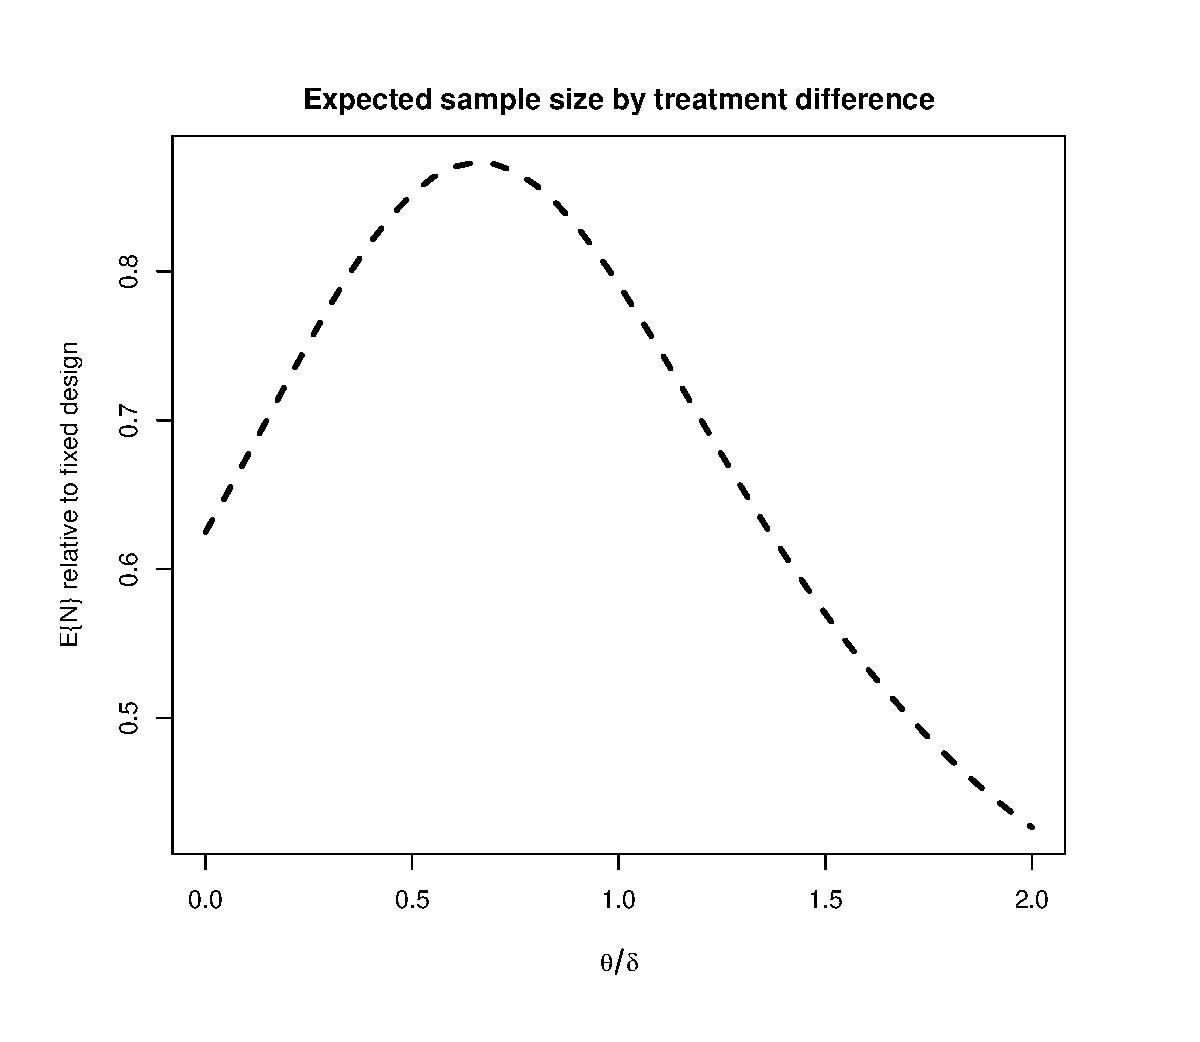
\includegraphics[width=.6\textwidth]{figs/ASN.pdf}
\end{center}
\caption{Average sample size plot}
\end{figure}
